\documentclass[border=10pt]{standalone}
\usepackage{amsmath}
\usepackage{tikz}
\usetikzlibrary{arrows.meta, calc, shapes.misc}

\begin{document}
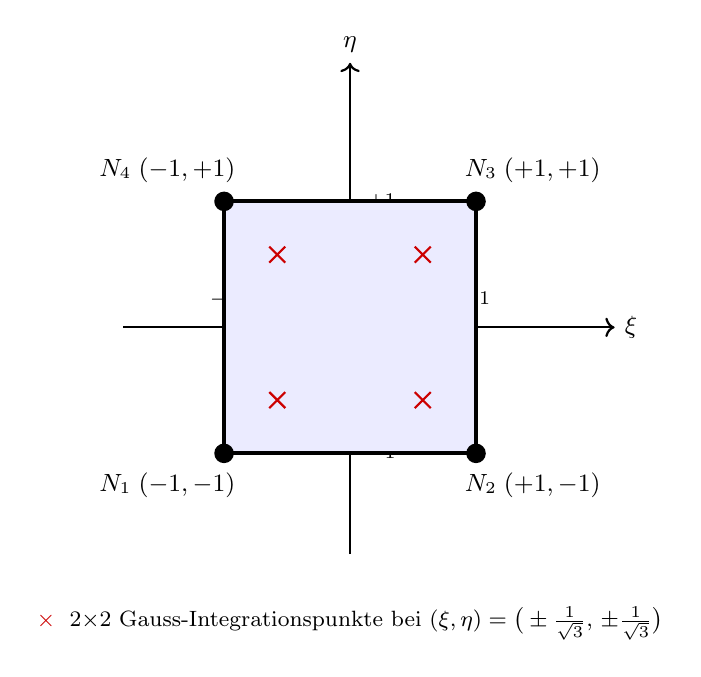
\begin{tikzpicture}[scale=1.6, every node/.style={font=\small},
    axis/.style={->, thick, black},
    edge/.style={line width=1.4pt, black},
    node_dot/.style={circle, fill=black, inner sep=2.5pt},
    nodelabel/.style={font=\bfseries\small},
    gausspt/.style={cross out, draw=red!80!black, thick, inner sep=2.5pt}
  ]

  % Achsen
  \draw[axis] (-1.8, 0) -- (2.1, 0) node[right] {$\xi$};
  \draw[axis] (0, -1.8) -- (0, 2.1) node[above] {$\eta$};

  % Tick-Marken an den Achsen, Labels weit nach aussen
  \draw[thick] (-1, 0.07) -- (-1, -0.07);
  \draw[thick] ( 1, 0.07) -- ( 1, -0.07);
  \draw[thick] (0.07, -1) -- (-0.07, -1);
  \draw[thick] (0.07,  1) -- (-0.07,  1);

  \node[font=\scriptsize] at (-1, 0.22) {$-1$};
  \node[font=\scriptsize] at ( 1, 0.22) {$+1$};
  \node[font=\scriptsize] at (0.25, -1) {$-1$};
  \node[font=\scriptsize] at (0.25,  1) {$+1$};

  % Referenzquadrat
  \draw[edge, fill=blue!8] (-1, -1) rectangle (1, 1);

  % Gauss-Punkte (2x2) bei +- 1/sqrt(3)
  \pgfmathsetmacro{\g}{0.5774}
  \node[gausspt] at (-\g, -\g) {};
  \node[gausspt] at ( \g, -\g) {};
  \node[gausspt] at (-\g,  \g) {};
  \node[gausspt] at ( \g,  \g) {};

  % Eckknoten mit Punkten und Beschriftung (weiter weg vom Knoten)
  \node[node_dot] at (-1, -1) {};
  \node[node_dot] at ( 1, -1) {};
  \node[node_dot] at ( 1,  1) {};
  \node[node_dot] at (-1,  1) {};

  \node[nodelabel] at (-1.45, -1.25) {$N_1\;(-1,-1)$};
  \node[nodelabel] at ( 1.45, -1.25) {$N_2\;(+1,-1)$};
  \node[nodelabel] at ( 1.45,  1.25) {$N_3\;(+1,+1)$};
  \node[nodelabel] at (-1.45,  1.25) {$N_4\;(-1,+1)$};

  % Legende unter dem Bild
  \node[align=center, font=\footnotesize] at (0, -2.35) {%
    \textcolor{red!80!black}{$\times$}\;
    2$\times$2 Gauss-Integrationspunkte
    bei $(\xi,\eta) = \big(\pm\tfrac{1}{\sqrt{3}},\,\pm\tfrac{1}{\sqrt{3}}\big)$%
  };

\end{tikzpicture}
\end{document}
